% You can choose whether you prefer a single or double column appendix.
% Whatever you choose, you will need to stick to it throughout the appendix.
% For double column style, comment the next line.
\onecolumn

\appendix
\begin{appendices}

\section{Acknowledgements}
\label{sec:apx:first_appendix}

My sincere gratitude to all the participants who generously contributed to this study by dedicating their time to respond to the surveys and questionnaires voluntarily, as well as those who willingly tested and interacted with the prototype. Special appreciation goes to everyone who supported me in data analysis, provided hardware for the prototypes, and reviewed and tested the code for the hardware devices.

A thank you to supervisor, Dr. H. Seiied Alavi (University of Amsterdam), for his invaluable guidance, though-provoking questions, and overall assistance throughout the project and Dr. Shruti Rao (University of Amsterdam) for her constructive feedback and suggestions, which further expanded this research. Also, my sincere appreciation to all the reviewers of this research for their insightful comments and contributions.

\section{Ethical considerations}
\label{sec:apx:first_appendix}

Before user studies were conducted, an application to the Ethics Committee for Information Sciences (ECIS) \footnote{https://ivi.uva.nl/research/ethical-code/ethical-code.html} about the methodology of this research, how data is being gathered and stored was made. Advice from the committee is still pending.

Prior to conducting the questionnaire survey and evaluation procedure, a domain expert from the Informatics Institute at the University of Amsterdam reviewed the methodologies involved. All individuals participating in the survey and evaluation process were obliged to confirm their voluntary involvement by carefully reading and signing a letter of consent, with the assurance that they retained the right to withdraw from participation at any point without the need for explanation. To uphold confidentiality and privacy, survey participation occurred anonymously, and all evaluation data underwent anonymization following the conclusion of the evaluation sessions.

Interacting with occupants within the building and interacting with participants of the usability tests of the prototype adhered to the the principles outlined in the UvA code of conduct \footnote{https://www.uva.nl/en/about-the-uva/policy-and-regulations/}.

\section{Data storage and archival}
\label{sec:apx:first_appendix}

Take some parts of the ethical application to describe data storage and archival of the devices etc.

\section{Source code}

In the spirit of open research, to support reproducibility and enable future work in this problem space the datasets, research notebooks, and prototypes in this work are publicly available on a GitHub organization with the working title 'viszlab' \footnote{https://github.com/viszlab} using the MIT License. Several code repositories for different parts of the research can be accessed. The readme.md of the repository described the contents and how to perform the technical set-up:

\begin{enumerate}
  \item \textbf{Prototype}. Code and models for the physical prototype.\\
  \underline{https://github.com/viszlab/prototype}
  \item \textbf{Datasets}. Code and models for the physical prototype.\\
  \underline{https://github.com/viszlab/prototype}
\end{enumerate}

A one-page website was created for shareability of this research. It's an online website which gives an overview of the research, allows for viewing the source coded of the prototype and allows for downloading of this paper. A live version is deployed on:

\begin{enumerate}
  \item \textbf{One-pager}. Code and models for the physical prototype.\\
  \underline{https://viszlab.github.io/}
\end{enumerate}

\pagebreak

\section{Floorplan and lab set-up}
\label{sec:apx:first_appendix}

A diagram indicating where the sensors where installed. This shows the lab set-up in the two meeting rooms.

\begin{figure}[H]
    \centering
    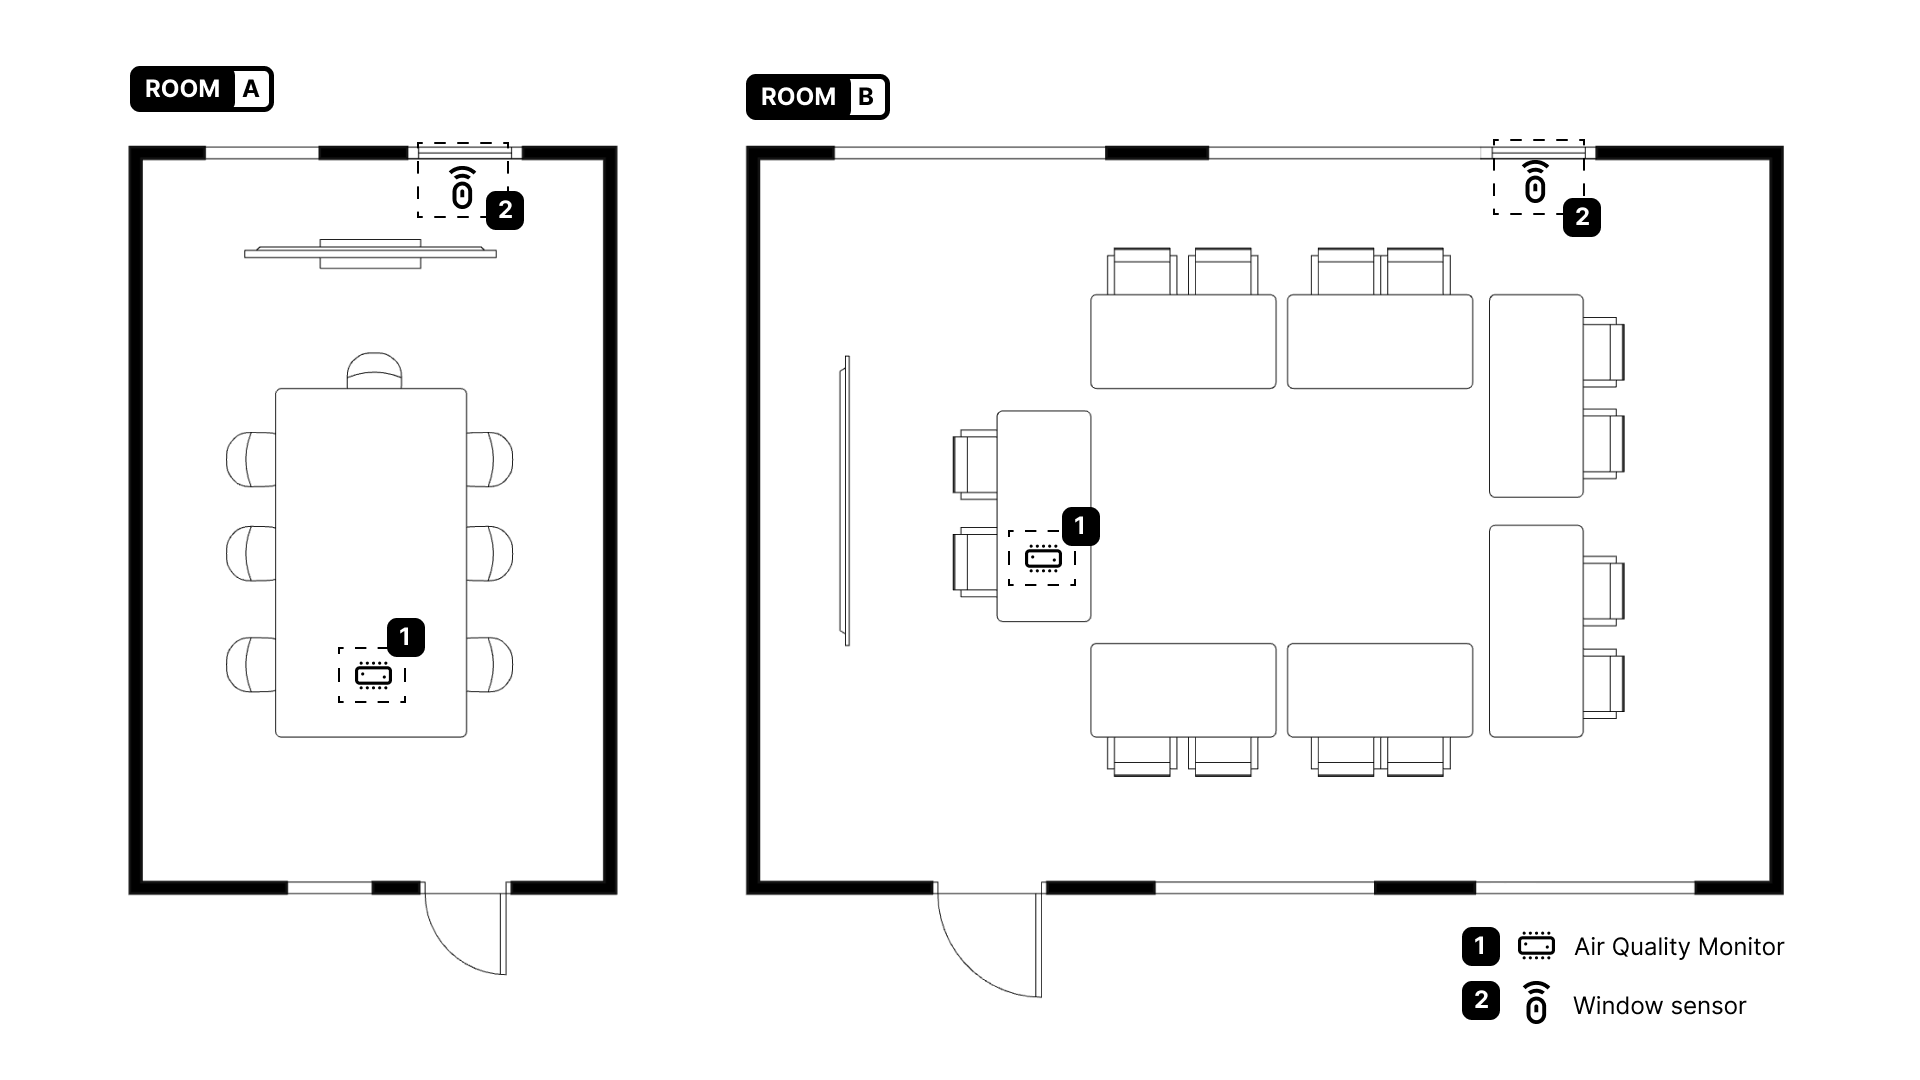
\includegraphics[width=0.6\paperwidth]{floorplan.png}
    \caption{Diagram of the floorplan with sensors installed}
    \label{fig:timeline}
\end{figure}

\section{IoT architecture of the prototype}
\label{sec:apx:first_appendix}

System diagram which shows the IoT architecture of the prototype.

\begin{figure}[H]
    \centering
    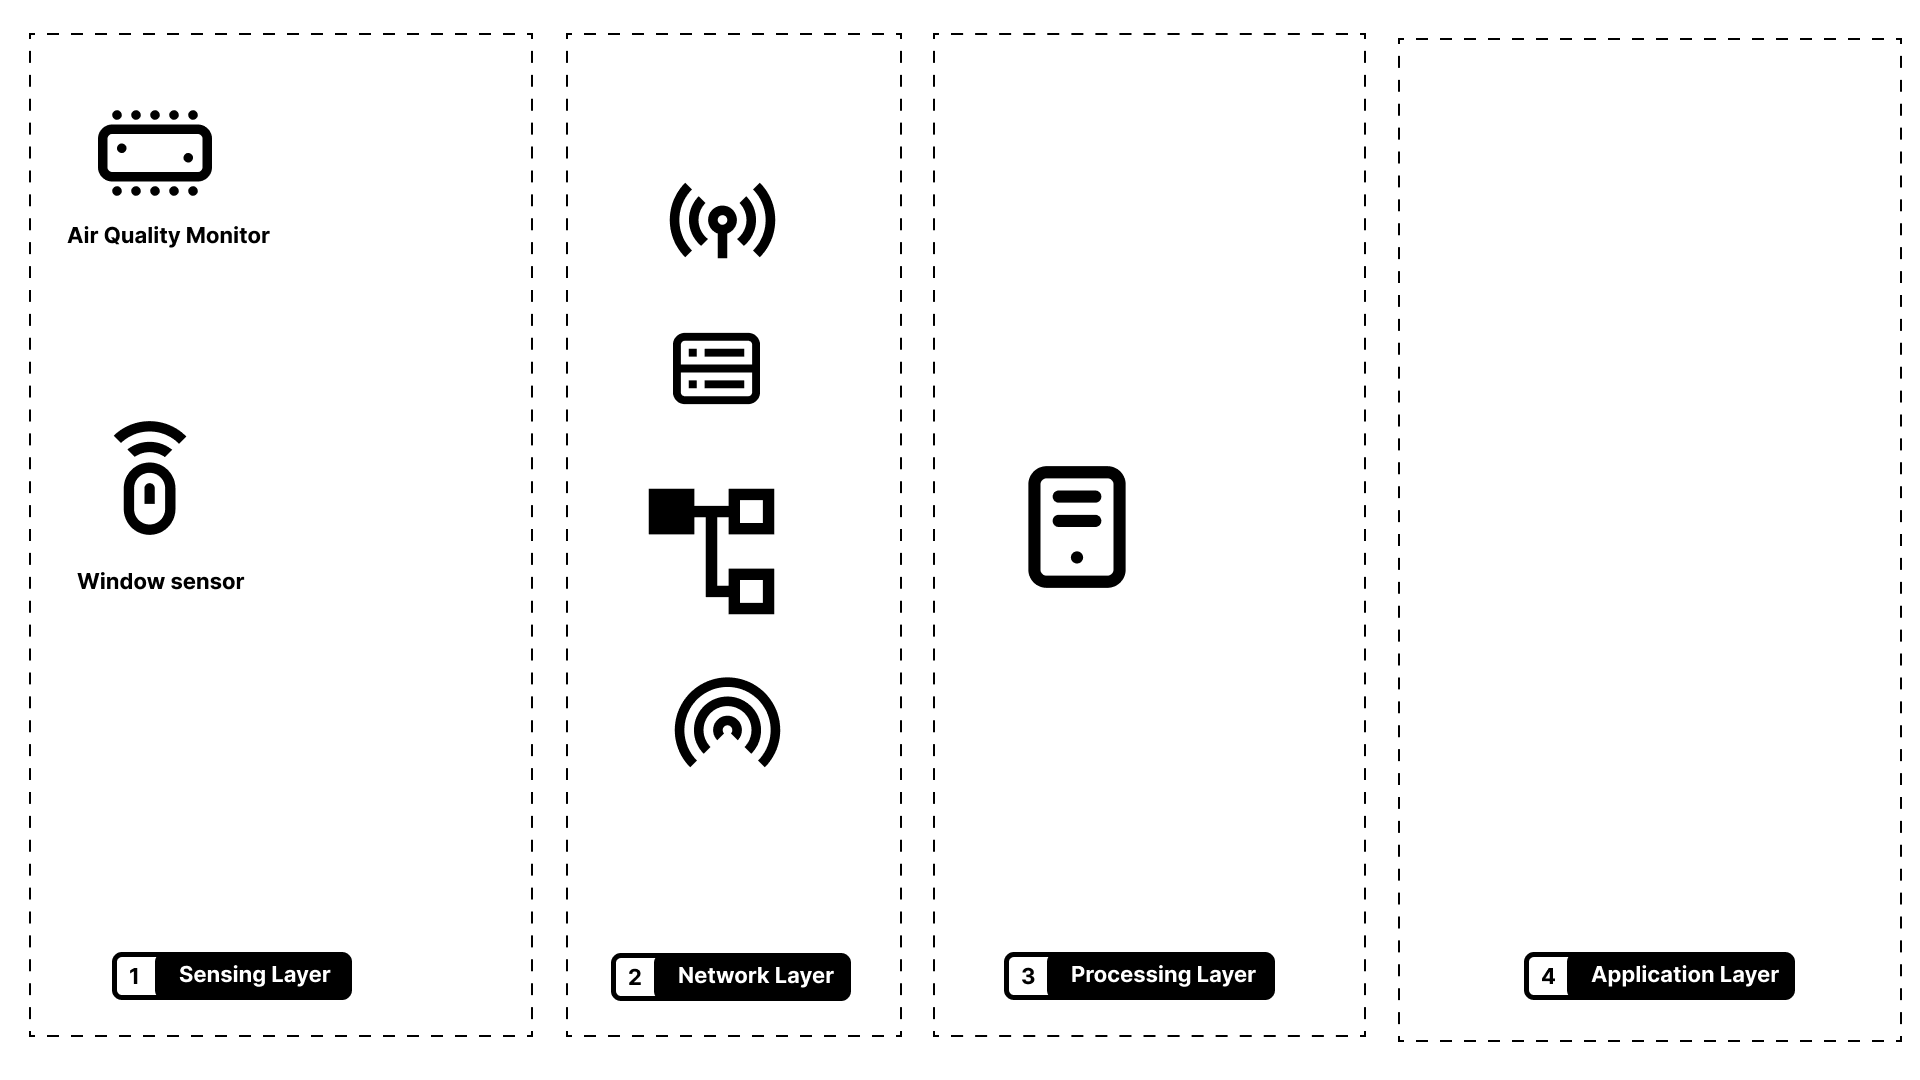
\includegraphics[width=0.7\paperwidth]{system.png}
    \caption{System diagram that shows the technical set-up of the prototype}
    \label{fig:timeline}
\end{figure}

\pagebreak

\section{Meeting room impressions}
\label{sec:apx:first_appendix}

\begin{figure}[H]
\begin{minipage}{.5\textwidth}
    \centering
    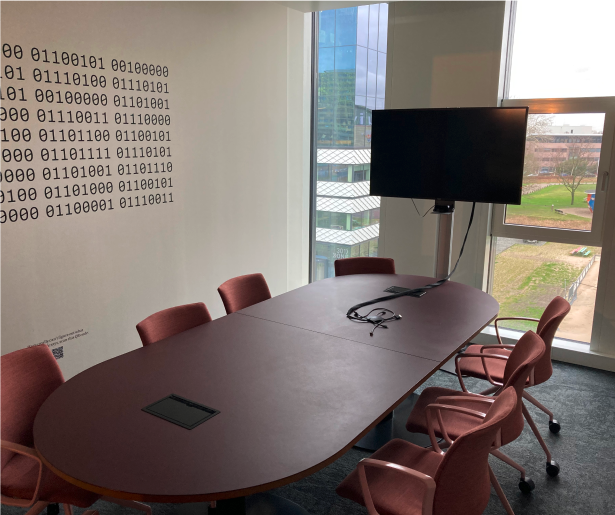
\includegraphics[width=80mm,height=80mm]{building.png}
    \caption{System diagram that shows the }
    \label{fig:timeline}
\end{minipage}%
\begin{minipage}{.5\textwidth}
    \centering
    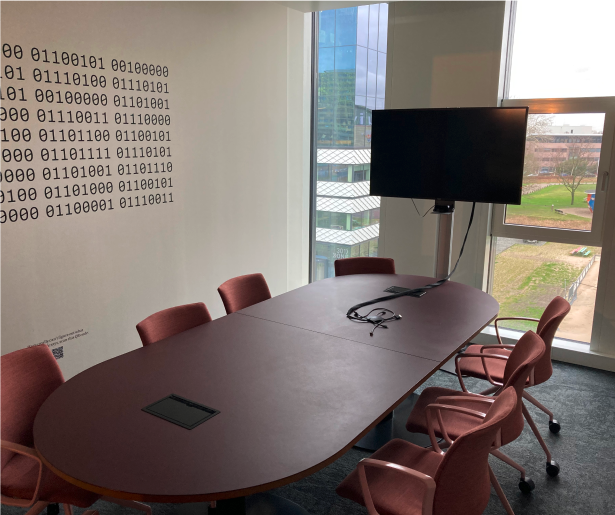
\includegraphics[width=80mm,height=80mm]{building.png}
    \caption{System diagram that shows the }
    \label{fig:timeline}
\end{minipage}%
\end{figure}

\section{Building impressions}
\label{appendix:building}

\begin{figure}[H]
\begin{minipage}{.5\textwidth}
\begin{tabular}{cc}
  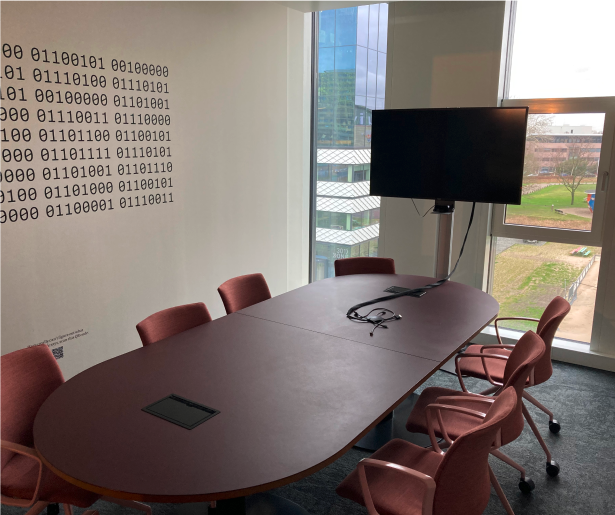
\includegraphics[width=45mm]{building.png} &   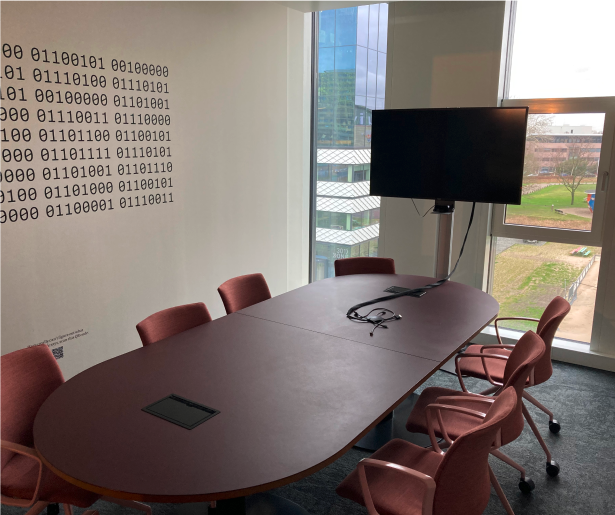
\includegraphics[width=45mm]{building.png} \\
(a) first & (b) second \\[6pt]
 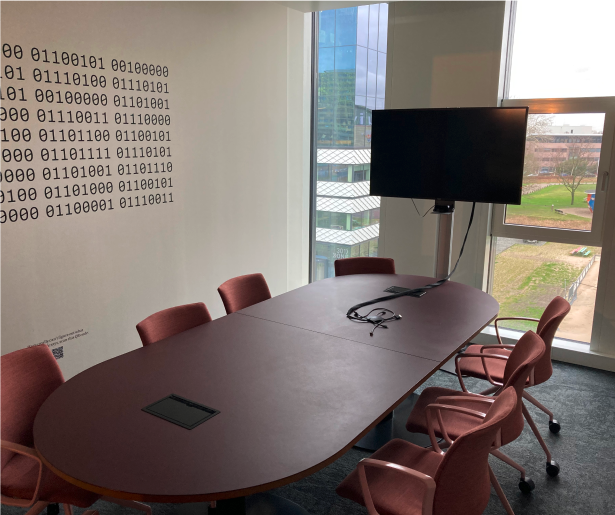
\includegraphics[width=45mm]{building.png} &   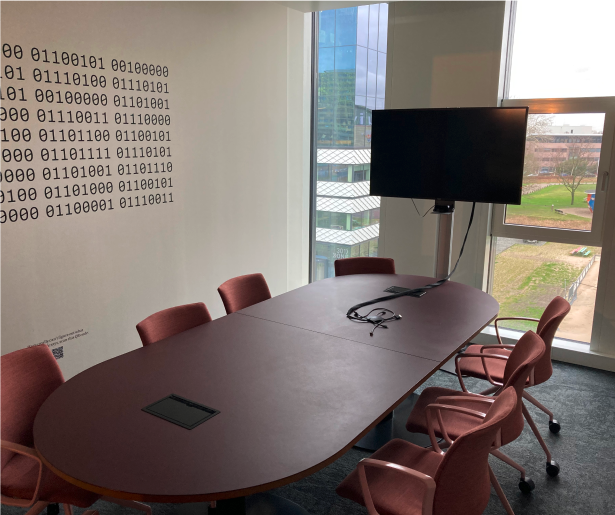
\includegraphics[width=45mm]{building.png} \\
(c) third & (d) fourth \\[6pt]
\end{tabular}
\caption{caption}
\end{minipage}%
\begin{minipage}{.5\textwidth}
    \centering
    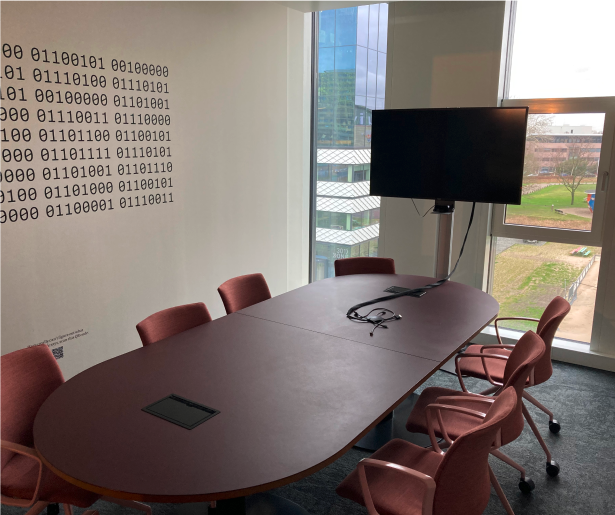
\includegraphics[width=70mm,height=80mm]{building.png}
    \caption{System diagram that shows the }
    \label{fig:timeline}
\end{minipage}%
\end{figure}

\section{Prototype impressions}
\label{sec:apx:first_appendix}

\begin{figure}[H]
\begin{minipage}{.5\textwidth}
    \centering
    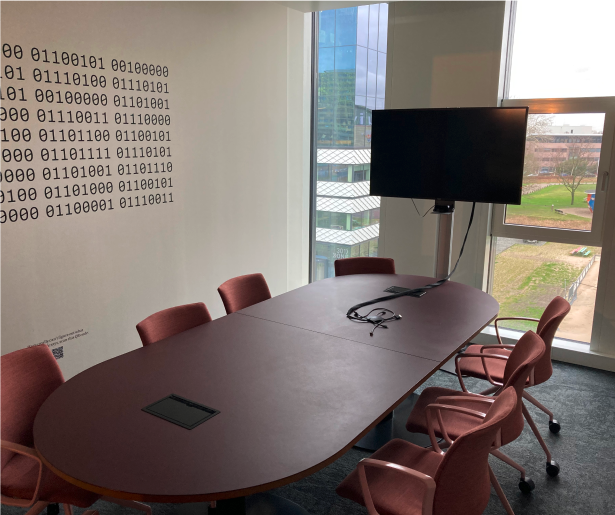
\includegraphics[width=70mm,height=80mm]{building.png}
    \caption{System diagram that shows the }
    \label{fig:timeline}
\end{minipage}%
\begin{minipage}{.5\textwidth}
\begin{tabular}{cc}
  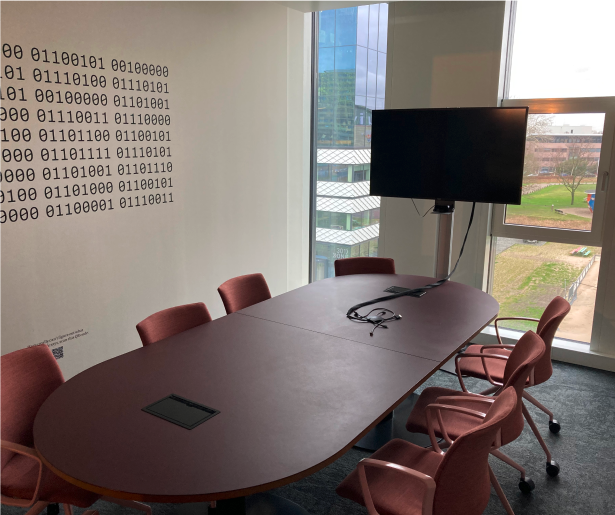
\includegraphics[width=45mm]{building.png} &   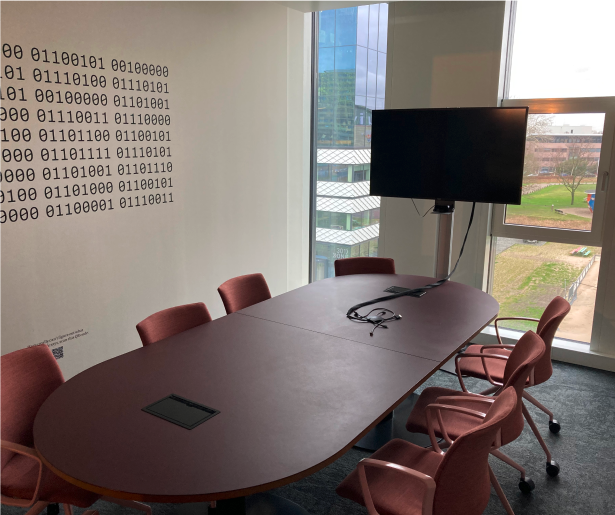
\includegraphics[width=45mm]{building.png} \\
(a) first & (b) second \\[6pt]
 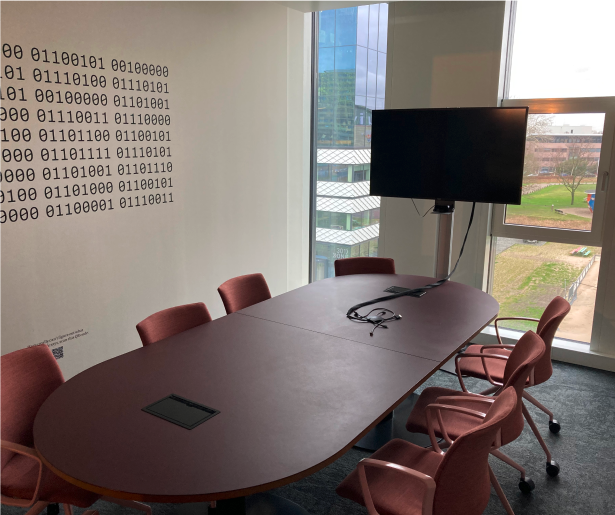
\includegraphics[width=45mm]{building.png} &   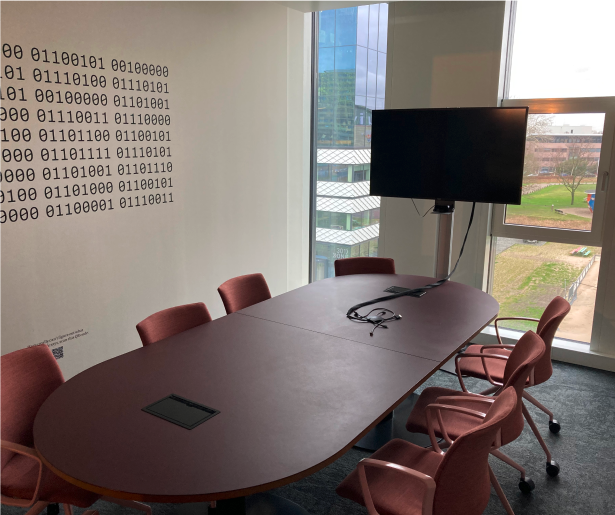
\includegraphics[width=45mm]{building.png} \\
(c) third & (d) fourth \\[6pt]
\end{tabular}
\caption{caption}
\end{minipage}%
\end{figure}

\section{Weekly schedule}
\label{sec:apx:first_appendix}

Horizontal boxplot that indicates an average week of booking in the meeting rooms scheduled.

\begin{figure}[H]
    \centering
    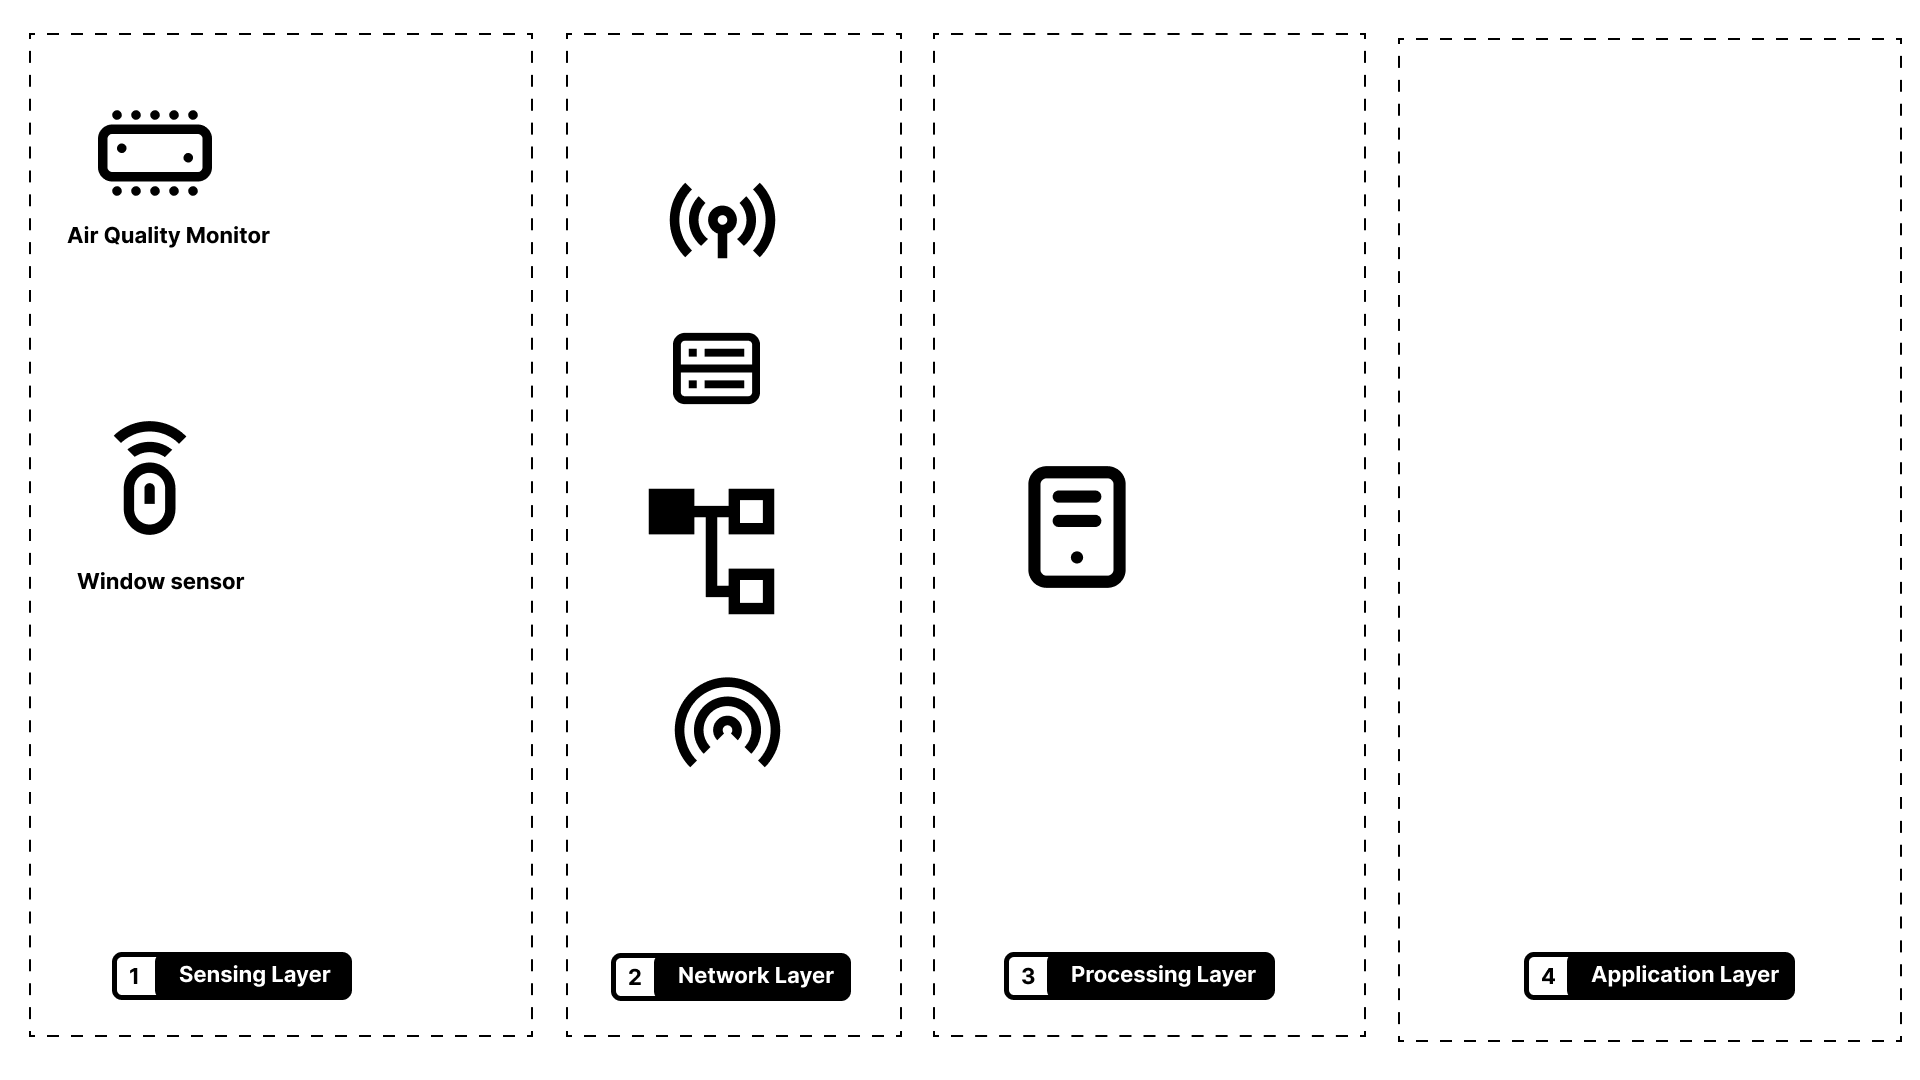
\includegraphics[width=0.7\paperwidth]{system.png}
    \caption{System diagram that shows the technical set-up of the prototype}
    \label{fig:timeline}
\end{figure}

\pagebreak

\section{Air Quality Monitors sample data}
\label{sec:apx:first_appendix}




\end{appendices}
